\documentclass[]{article}


\author{Silvio Gregorini}
\title{}
\date{2019}

% Ask if it's possible to use a two column layout
\usepackage[utf8]{inputenc}
\usepackage{csquotes}
\usepackage[english]{babel}
\usepackage{xcolor}
\usepackage[urlbordercolor=white, linkbordercolor=white, citebordercolor=white]{hyperref}
\usepackage{graphicx}
%\usepackage[style=authoryear]{biblatex}
%\addbibresource{bibliography.bib}

\newcommand{\bibTitle}[1]{\emph{#1}}
\newcommand{\bibYear}[1]{(#1)}
\newcommand{\bibUrl}[1]{\textless#1\textgreater}
\newcommand{\bibUrldate}[1]{[Accessed #1]}

\newcommand{\citeInText}[2]{#1 (#2)}

% Change appearance of numeric labels in citation call-outs
\usepackage{cite}
\renewcommand\citeleft{(}
\renewcommand\citeright{)}

% Change appearance of numeric labels in bibliography 
\makeatletter
\renewcommand{\@biblabel}[1]{}
\makeatother

%\renewcommand{\urlbordercolor}{0} {0} {0}

\begin{document}

%================================================================================
%PUT NUMBERS ON PARAGRAPHS

\section{Introduction} %DONE

    The aim of this paper is to propose the design and production of an 
    hardware synthesizer, starting from an existing digital sound engine.
    In the sections that follow, it will be explained the background and the rationale 
    behind the project, as well as the initial research undertaken.
    Then, it will be depicted a "blueprint" of the product: the general concept, the 
    architecture of the system -- both hardware and software -- and the production plan 
    will be covered in detail.
    In the last part the evaluation criteria will be set, in order to have a concrete measure
    of the work outcomes.

\section{Background and Motivation}

    This project has been shaped and will be realised keeping as a pivotal point the
    \emph{chiptune} subculture and its principles. As will be discussed in the next paragraphs,
    the product is conceived to be used by people already familiar with the environment and 
    limitations of this musical style. Its purpose is to give users a different and more 
    modern way to interact with a well-known set of sounds and synthesis capabilities.

    \subsection{Pushing the Limits Using Contraints} %_______________________________________________________________________________________________________CITE TEDX DAN BEHERENS
        \paragraph{Chiptune} %DONE
        As stated by Collins et al. (2014 )\nocite{COLLINS2014} the term \emph{chiptune} has multiple 
        definitions. Also known as \emph{chip music} or \emph{8-bit music}, it derives from the sound chips that,
         in the first generation of computers and gaming consoles,
         were used to balance the processing power of generating sound effects and music from the
        CPU. In its strictiest meaning, chiptune is used to refer to music created entirely from the original, vintage audio 
        chips. Nevertheless, modifications that do not alter the nature of the sound produced are allowed.\\
        The broadest definition is more related to the aesthetics of the sound, rather then to the source
        generating it. The entire subculture which gravitates around the foundations and features of chip
        music can be called \emph{chiptune} too. Anyway, this paper and the related project will try to stick
        to the strictiest definition of the word, in order to create a product able to maintain the sound fidelity
        of the old processors.

        \paragraph{DMG-001 and trackers} %DONE
        In particular, the following study focuses on the Nintendo DMG-001 from 1989, known with the commercial 
        name of \emph{Game Boy}, which is supposedly one of the most popular tools for the production of chip music.
        From the official datasheet (Nintendo, 2019)\nocite{NINTENDO2019} portable console runs on a custom 
        \emph{Sharp LR35902} 8-bit CPU, similar to the \emph{Zilog Z80}\footnote{Popular 8-bit microprocessor widely used 
        from the 1970s to the mid-1980s in desktop and home computers, military applications, synthesizers, arcade machines\ldots} 
        and has four audio channels\footnote{To be precise, as stated in the 8BC Chiptune Wiki (2007)\nocite{8BCCHIPTUNE2007}, 
        the console has a fifth -- and least known -- channel: it is an analogue input channel that allows 
        external synthesis on cartridge to be mixed with the sound generated by the other channels. No cartridges 
        are known to use this channel and its functionality, though.}:\\[10pt]
        
        \def\arraystretch{1.2}
        \begin{tabular}{l l l}
            \hline
            \textbf{Channel} & \textbf{Type} & \textbf{Features}\\
            \hline \\[-6pt]
            1 & Quadrangular\footnotemark & - Volume envelope\\
                &   &                                                                          - 4-mode pulse width\\
                &   &                                                                          - Frequency register from C3 upwards\\
                &   &                                                                          - Frequency envelope\\            
            \hline
            2 & Quadrangular & - Volume envelope\\       
            &   &              - 4-mode pulse width\\
            &   &              - Frequency register from C3 upwards\\
            \hline
            3 & Wave & - User-definable waveforms\\
            &   &      - Bank of 32 samples (4-bit each)\\
            &   &      - Frequency register from C2 upwards\\
            \hline
            4 & Pseudo-random noise & - White and brown noise\\
            \hline \\
        \end{tabular}
        \footnotetext{Also known as \emph{pulse wave} or \emph{square wave}.}
        
        \nocite{MARQUEZ2014}

        Back in the analog era (i.e. before the first DAWs were created and deployed), the tools to compose and produce music on digital 
        computers and consoles were the \emph{music trackers}. They can be defined as precursors of the modern 
        music production softwares: notes, parameters, effects and other commands, in this type of vertical sequencer, are given
        as letters, numbers or hexadecimal digits into a fixed, time-slotted grid. Fig.\ref{fig:lsdj} shows an
        example of a tracker interface: \emph{Little Sound Dj}, the most popular music editor for 
        Game Boy consoles. The implementation of this tracker, along with other softwares like \emph{nanoloop} 
        and \emph{mGB}, will be considered in the design of the proposed product. \\

        \begin{figure}[h]
            \centering
            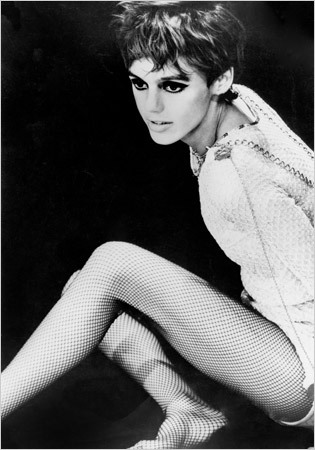
\includegraphics[width=.5\textwidth]{PLACEHOLDER.jpg} %_______________________________________________________________________________________________________LSDJ PICTURE
            \caption{\emph{Song} Screen on the popular LSDJ tracker for Game Boy \cite{KOTLINSKI2007}}
            \label{fig:lsdj}
        \end{figure}


    \subsection{Rationale}  %_______________________________________________________________________________________________________NAME
            Despite being one of the cardinal points in the \emph{Chiptune} subculture, the idea of 
            maintaning the limitations given by the hardware is too general and vague, and a distinction is 
            necessary. During the composition and execution of 8-bit music, two main types of constraints can be addressed:

            \begin{itemize}
            \item \textbf{Processing capabilities} -- The true and interesting challenge, i.e. to try to push the 
                    hardware CPU to its limit, creating complex sounds and tracks on a level that was considered 
                    unachievable, given the limited digital resources.
            \item \textbf{User interface} -- Even though someone could disagree with this opinion, from a practical view, limitations in the UI
                    can be considered nothing more than an obstacle in the production process. If we take the DMG-001 as an example, being constrained
                    by a D-pad and four push buttons has nothing to share with the concept of taking out deep and articulated music from a 4.19 MHz CPU with 8 KB of RAM.
            \end{itemize}

            So, it is clear that a limitation in the UI is unnecessary and -- most of the time -- unwanted. For this reasons, the aim 
            behind the proposed product is to renew the link between chiptune musicians and instruments, expanding the interactive capabilities of the Game Boy, 
            without perverting the characteristic soundscape and the core aspects of its composition process.

\section{Name of the Project}  %_______________________________________________________________________________________________________NAME
    \subsection{Concept}
    \subsection{System Architecture}
        \paragraph{Hardware}
            \subparagraph{Controls}
            \subparagraph{User Interface}
        \paragraph{DMG-001 Mods}
            \subparagraph{Sound}
            \subparagraph{Midi Functionality}
            \subparagraph{Screen}
            \subparagraph{Power}
        \paragraph{Embedded Software}
    \subsection{Production}
        \paragraph{Resources}
        \paragraph{Schedule}

\section{Discussion}
    \subsection{Minimum Viable Product}
    \subsection{Evaluation Criteria}

\section{Conclusions}



%=================================================%
%       REMEMBER TO SORT THE BIBLIOGRAPHY
%=================================================%

\begin{thebibliography}{99}

    \bibitem[Collins et al., 2014]{COLLINS2014}
    Collins, K. and Kapralos, B. and Tessler, H. and Paul, J. L.
    \bibYear{2014}
    \bibTitle{The Oxford Handbook of Interactive Audio.}
    USA: Oxford University Press.

    
    \bibitem[Marquez, 2014]{MARQUEZ2014}
    Marquez, I.
    \bibYear{2014}
    Playing new music with old games: The chiptune subculture.
    \bibTitle{G| A| M| E Games as Art, Media, Entertainment}
    [Online], 1 (3), pp. 67-79. Available from: 
    \bibUrl{\url{http://www.gamejournal.it/wp-content/uploads/2014/04/GAME_3_Subcultures_Journal_Marquez.pdf}}
    \bibUrldate{20 October 2019}.


    \bibitem[Nintendo, 2019]{NINTENDO2019}
    Nintendo
    \bibYear{2019}
    \bibTitle{Game Boy, Game Boy Color, Game Boy Pocket Technical Data}
    [Support page] [Online] Available from: 
    \bibUrl{\url{https://www.nintendo.co.uk/Support/Game-Boy-Pocket-Color/Product-information/Technical-data/Technical-data-619585.html}}
    \bibUrldate{20 October 2019}.

\end{thebibliography}




%================================================================================

In this module, you will develop an original interactive or reactive system
in which music or sound is a key component. Innovative and imaginative
 methods of interaction by a participant should be explored, and this
  could be for any relevant context (performance, composition, installation,
   game, sound toy, etc).
   
During the first half of the module, you should consider and develop a 
written proposal and plan for this project. Your proposal should be around 
2000 words and address the following areas:

\subparagraph[]{Section 1}
    \textbf{Overall project aims and rationale Who is your project aimed at?}

    \textbf{In what situation/context is it designed to be used?}
    
        \begin{itemize}
        \item Live performance
        \item Music production
        \end{itemize}

    \textbf{How and why will people engage with it?}

        \begin{itemize}
        \item It will be an easy and straightforward way of making chiptune music
        \end{itemize}

\subparagraph[]{Section 2}

    \textbf{Details of project What are the key hardware/software elements in your
    project?}

        \begin{itemize}
            \item Sound engine: GameBoy DMG-01 (1989)
            \item New Hardware Interface
        \end{itemize}

    \textbf{What sounds will your system work with?}
    The system will generate sound using the sound chip of the GameBoy

    \textbf{What will the relationship be between user inputs and the sound 
    parameters (mapping)?} 
    To interact with the sound, the Midi protocol will be used.
    Since the GameBoy can't read and understand Midi messages,
    a translation unit is required amid the interface and the sound engine (i.e. an Arduino board).

    \textbf{How does this mapping support your overall project aims?}

\subparagraph[]{Section 3}

    \textbf{Evidence of contextual awareness, research and reading What other similar
    systems have you looked at? How has your idea developed from this research? }
    
    \textbf{What relevant concepts have fed into your design process?}

\subparagraph[]{Section 4}
    
    \textbf{Plan for implementation What resources do you require to complete your
    project? What specific tasks do you need to complete and by when?}

    \textbf{This should be written using appropriate academic language with reference
    to relevant texts/media using Harvard format.}

%    And this is my first resource: \cite{kevin}


%\printbibliography

\end{document}

